\chapter{Results and Discussion}

\section{Operational KPIs from the Deployed System}
Table~\ref{tab:kpis} lists the KPIs reported by the live system's analytics module for the Chennai DC over the 30 days from 6 October to 4 November 2026. The appointments in this period come from the demo data generator, which models five carriers with different punctuality profiles, morning and afternoon demand peaks, and realistic gate-to-dock and handling times. The figures therefore demonstrate what the system measures and how; they are not measurements from a real warehouse.

\begin{table}[H]
\centering
\caption{KPIs reported by SmartDock (Chennai DC, 30 days, demo data)}
\label{tab:kpis}
\begin{tabular}{lr@{\hspace{2.5em}}lr}
\toprule
\textbf{KPI} & \textbf{Value} & \textbf{KPI} & \textbf{Value}\\
\midrule
Appointments & 910 & Average per day & 30.3 \\
Completed & 799 & Pallets handled & 15{,}151 \\
Dock utilisation & 40.0\% & Offered truck-slots & 2{,}184 \\
On-time arrival rate & 78.6\% & No-show rate & 8.6\% \\
Cancellation rate & 4.0\% & Avg.\ turnaround (gate to gate) & 57 min \\
Avg.\ yard wait (gate to door) & 17 min & Avg.\ dock time (handling) & 40 min \\
\bottomrule
\end{tabular}
\end{table}

\paragraph{Discussion.} A 40\% utilisation with an 8.6\% no-show rate shows that capacity is available but is partly reserved by trucks that never arrive --- a direct, quantified case for the waitlist (which reallocates released capacity) and for using the reliability score in carrier negotiations. The demand heatmap (Figure~\ref{fig:s-heat}) and busiest hours (10:00--11:00 and 15:00--16:00) show where labour should be concentrated and which hours carriers could be steered away from. The split of turnaround into a 17-minute yard wait and a 40-minute dock time tells the manager whether to work on gate and yard flow or on dock productivity.

\begin{figure}[H]
\centering
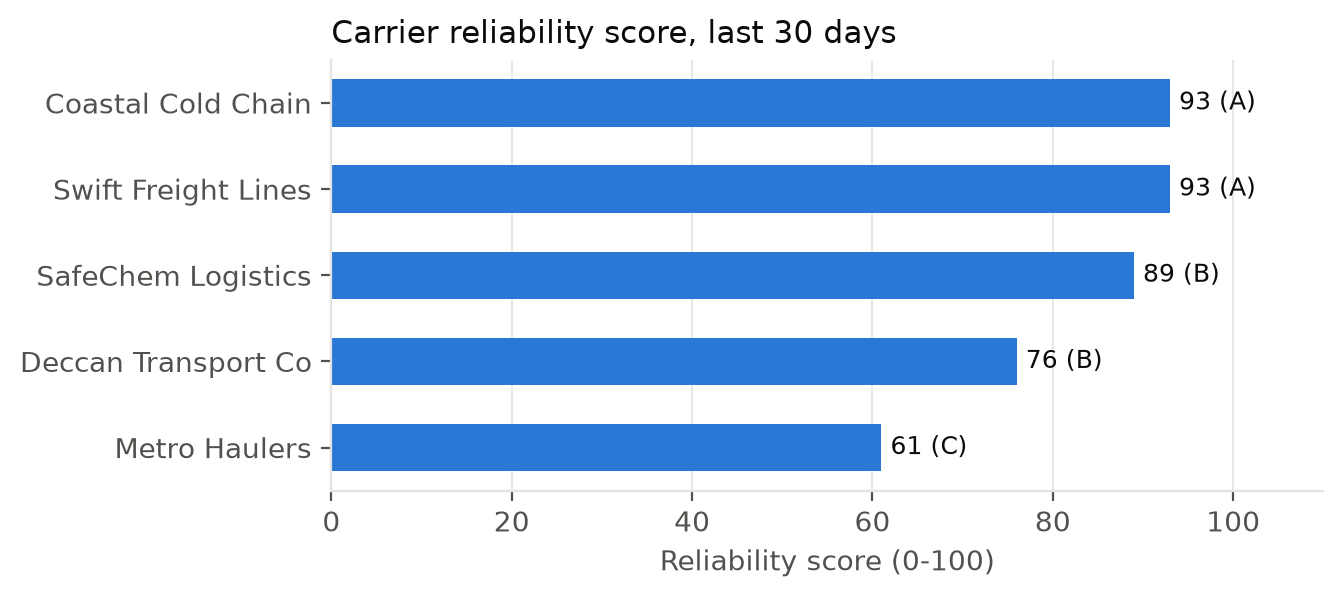
\includegraphics[width=0.85\textwidth]{fig_carrier_reliability.png}
\caption{Carrier reliability scores computed by the system}
\label{fig:rel}
\end{figure}

Figure~\ref{fig:rel} shows how the scorecard separates carriers: Swift Freight Lines and Coastal Cold Chain score 93 (tier A) with on-time rates above 90\%, while Metro Haulers scores 61 (tier C) with a 58\% on-time rate and the most no-shows. These differences are exactly the input a procurement team needs for carrier selection and performance clauses.

\begin{figure}[H]
\centering
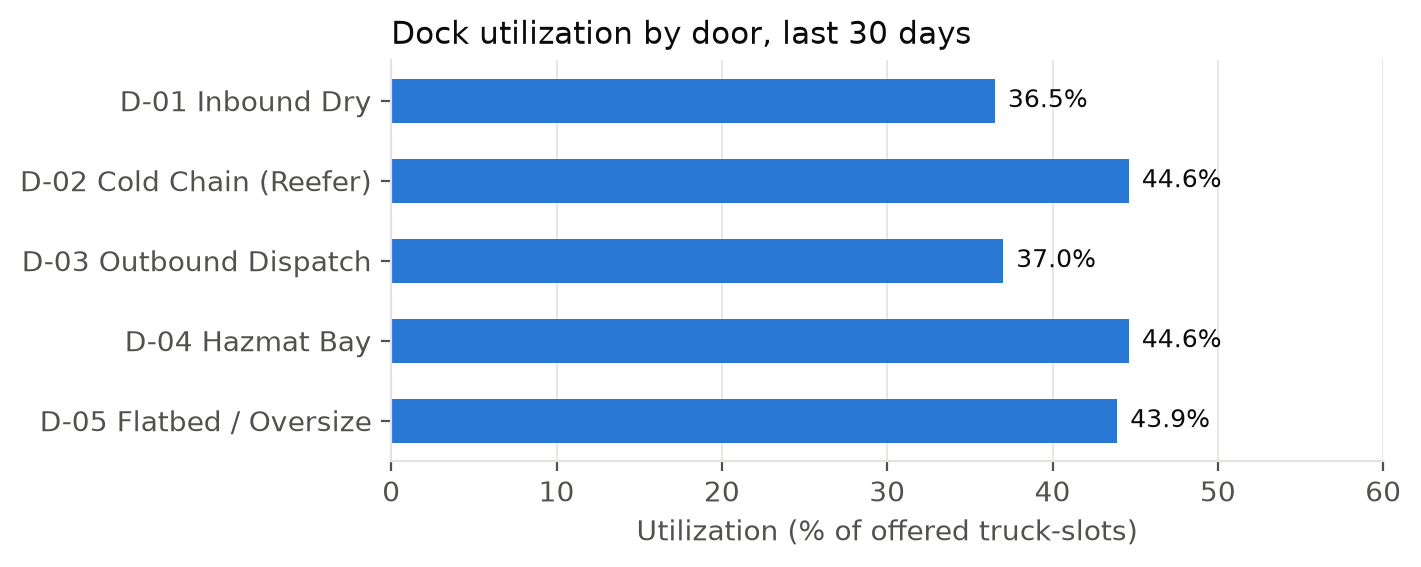
\includegraphics[width=0.85\textwidth]{fig_dock_utilization.png}
\caption{Utilisation by dock door}
\label{fig:dockutil}
\end{figure}

Single-capacity specialised doors (reefer, hazmat and flatbed, about 44--45\%) are relatively busier than the two-truck general doors (about 37\%), suggesting that specialised capacity, not total capacity, would become the constraint first as volume grows.

\section{Before-versus-After Comparison (Simulation)}
To estimate the effect of appointment scheduling on yard congestion, a discrete-event simulation \cite{law2015} was run (script \texttt{docs/analysis/make\_figures.py}). The model represents one DC day from 07:00 to 19:00 with six identical dock doors and 60 trucks; handling time is triangular (25, 40, 55 minutes) plus 5 minutes turnover; trucks are served first-come-first-served at the first free door. Sixty days were simulated for each scenario with the same random seed.

\begin{itemize}
  \item \textbf{Before (no appointments):} carriers arrive at their preferred time, drawn from a morning peak around 09:30 (55\%) and an afternoon peak around 14:30 (45\%).
  \item \textbf{After (SmartDock):} each carrier books the free 60-minute slot nearest its preferred time, with at most six trucks per slot (one per door), and arrives around the slot start with the punctuality mix observed in the demo data (80\% within $-15$ to $+12$ minutes, 15\% late by 16--55 minutes, 5\% no-show).
\end{itemize}

\begin{table}[H]
\centering
\caption{Simulated yard performance, 60 days per scenario}
\label{tab:sim}
\begin{tabular}{lrrr}
\toprule
\textbf{Metric} & \textbf{Before} & \textbf{After} & \textbf{Change}\\
\midrule
Mean wait from arrival to dock & 19.4 min & 1.0 min & $-95\%$\\
90th percentile wait & 54.9 min & 0.0 min & $-100\%$\\
Maximum wait observed & 116.3 min & 37.7 min & $-68\%$\\
Trucks waiting more than 30 min & 27.7\% & 0.3\% & $-27.4$ pts\\
Peak average yard queue & 7.0 trucks & 0.4 trucks & $-94\%$\\
\bottomrule
\end{tabular}
\end{table}

\begin{figure}[H]
\centering
\begin{subfigure}{0.49\textwidth}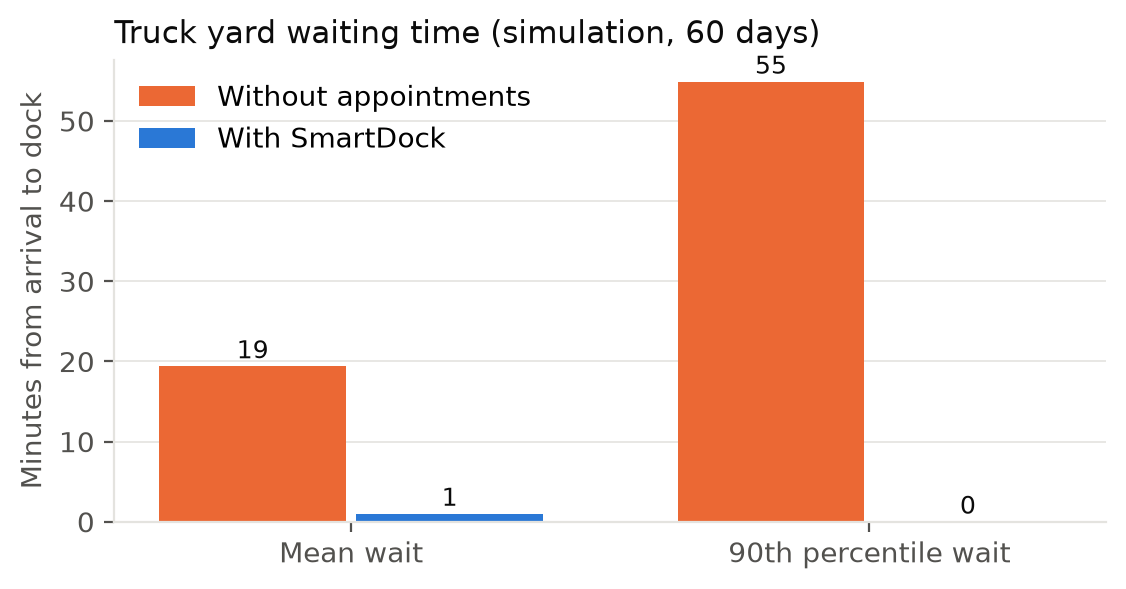
\includegraphics[width=\textwidth]{fig_sim_wait.png}\caption{Waiting time}\end{subfigure}
\hfill
\begin{subfigure}{0.49\textwidth}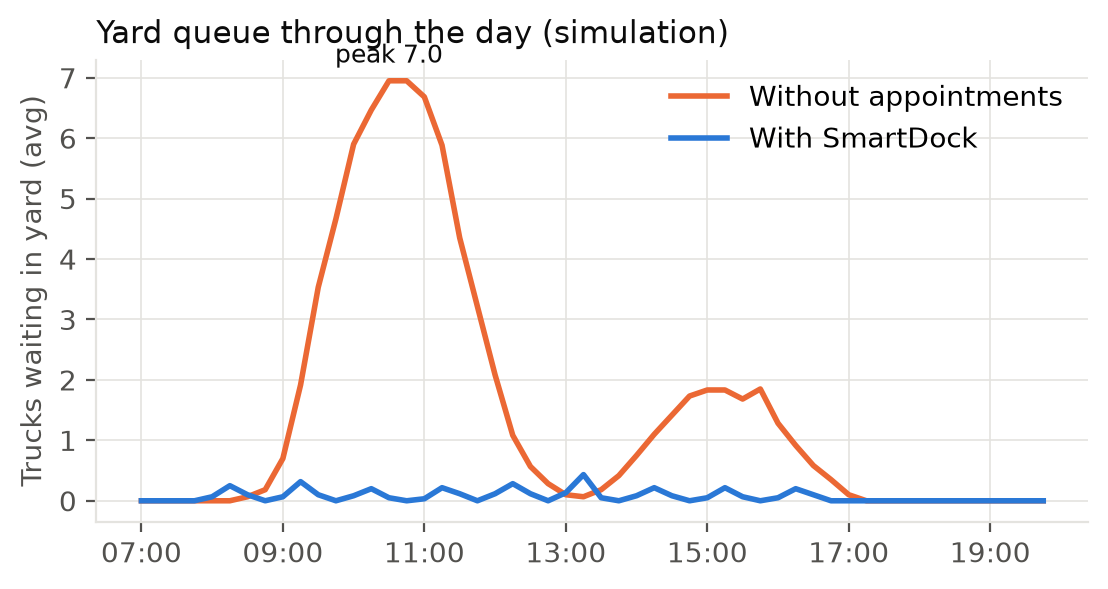
\includegraphics[width=\textwidth]{fig_sim_queue.png}\caption{Yard queue through the day}\end{subfigure}
\caption{Simulated effect of appointment scheduling}
\label{fig:sim}
\end{figure}

\paragraph{Discussion.} With the same docks and the same work, smoothing arrivals removes almost all queueing: the morning and afternoon peaks that create a queue of about seven trucks disappear because capacity is allocated before trucks arrive. The residual waits are caused by late trucks arriving while the next appointment is already at the door, which is precisely what the late-arrival tracking and reliability score are designed to discourage. In money terms, each truck-hour of waiting avoided reduces detention charges, driver hours and idling emissions --- the benefits reported for port appointment systems \cite{giuliano2007,zehendner2014}.

\paragraph{Threats to validity.} The simulation is deliberately simple: identical doors, one truck type, a fixed arrival pattern and perfect slot discipline for punctual trucks. In practice the gain depends on enforcement and carrier compliance \cite{giuliano2007}, on handling-time variability and on how peaky demand really is. The numbers should be read as an indication of the order of magnitude, to be confirmed by a pilot at a real site.

\section{Correctness Result}
The most important technical result is the double-booking experiment (Section~\ref{sec:concurrency}): under 40 simultaneous requests split across two servers, the naive approach admitted 15 trucks into a one-truck slot, whereas SmartDock admitted exactly one (and exactly three into a three-truck slot). For a warehouse this is the difference between a reliable schedule and a schedule that fails exactly at the busiest moments.
